\begin{frame}{Quantum Fourier transform}
	This is a well-known circuit:
	
	\pause 
	\begin{center}
		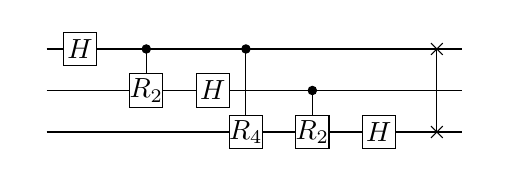
\begin{tikzpicture}[scale=1.000000,x=1pt,y=1pt]
\filldraw[color=white] (0.000000, -7.500000) rectangle (150.000000, 37.500000);
% Drawing wires
% Line 1: a W {} {}
\draw[color=black] (0.000000,30.000000) -- (150.000000,30.000000);
\draw[color=black] (0.000000,30.000000) node[left] {${}$};
% Line 2: b W {} {}
\draw[color=black] (0.000000,15.000000) -- (150.000000,15.000000);
\draw[color=black] (0.000000,15.000000) node[left] {${}$};
% Line 3: c W {} {}
\draw[color=black] (0.000000,0.000000) -- (150.000000,0.000000);
\draw[color=black] (0.000000,0.000000) node[left] {${}$};
% Done with wires; drawing gates
% Line 4: a H
\begin{scope}
\draw[fill=white] (12.000000, 30.000000) +(-45.000000:8.485281pt and 8.485281pt) -- +(45.000000:8.485281pt and 8.485281pt) -- +(135.000000:8.485281pt and 8.485281pt) -- +(225.000000:8.485281pt and 8.485281pt) -- cycle;
\clip (12.000000, 30.000000) +(-45.000000:8.485281pt and 8.485281pt) -- +(45.000000:8.485281pt and 8.485281pt) -- +(135.000000:8.485281pt and 8.485281pt) -- +(225.000000:8.485281pt and 8.485281pt) -- cycle;
\draw (12.000000, 30.000000) node {$H$};
\end{scope}
% Line 5: b G $R_2$ a
\draw (36.000000,30.000000) -- (36.000000,15.000000);
\begin{scope}
\draw[fill=white] (36.000000, 15.000000) +(-45.000000:8.485281pt and 8.485281pt) -- +(45.000000:8.485281pt and 8.485281pt) -- +(135.000000:8.485281pt and 8.485281pt) -- +(225.000000:8.485281pt and 8.485281pt) -- cycle;
\clip (36.000000, 15.000000) +(-45.000000:8.485281pt and 8.485281pt) -- +(45.000000:8.485281pt and 8.485281pt) -- +(135.000000:8.485281pt and 8.485281pt) -- +(225.000000:8.485281pt and 8.485281pt) -- cycle;
\draw (36.000000, 15.000000) node {$R_2$};
\end{scope}
\filldraw (36.000000, 30.000000) circle(1.500000pt);
% Line 6: b H
\begin{scope}
\draw[fill=white] (60.000000, 15.000000) +(-45.000000:8.485281pt and 8.485281pt) -- +(45.000000:8.485281pt and 8.485281pt) -- +(135.000000:8.485281pt and 8.485281pt) -- +(225.000000:8.485281pt and 8.485281pt) -- cycle;
\clip (60.000000, 15.000000) +(-45.000000:8.485281pt and 8.485281pt) -- +(45.000000:8.485281pt and 8.485281pt) -- +(135.000000:8.485281pt and 8.485281pt) -- +(225.000000:8.485281pt and 8.485281pt) -- cycle;
\draw (60.000000, 15.000000) node {$H$};
\end{scope}
% Line 7: c G $R_4$ a
\draw (72.000000,30.000000) -- (72.000000,0.000000);
\begin{scope}
\draw[fill=white] (72.000000, -0.000000) +(-45.000000:8.485281pt and 8.485281pt) -- +(45.000000:8.485281pt and 8.485281pt) -- +(135.000000:8.485281pt and 8.485281pt) -- +(225.000000:8.485281pt and 8.485281pt) -- cycle;
\clip (72.000000, -0.000000) +(-45.000000:8.485281pt and 8.485281pt) -- +(45.000000:8.485281pt and 8.485281pt) -- +(135.000000:8.485281pt and 8.485281pt) -- +(225.000000:8.485281pt and 8.485281pt) -- cycle;
\draw (72.000000, -0.000000) node {$R_4$};
\end{scope}
\filldraw (72.000000, 30.000000) circle(1.500000pt);
% Line 8: c G $R_2$ b
\draw (96.000000,15.000000) -- (96.000000,0.000000);
\begin{scope}
\draw[fill=white] (96.000000, -0.000000) +(-45.000000:8.485281pt and 8.485281pt) -- +(45.000000:8.485281pt and 8.485281pt) -- +(135.000000:8.485281pt and 8.485281pt) -- +(225.000000:8.485281pt and 8.485281pt) -- cycle;
\clip (96.000000, -0.000000) +(-45.000000:8.485281pt and 8.485281pt) -- +(45.000000:8.485281pt and 8.485281pt) -- +(135.000000:8.485281pt and 8.485281pt) -- +(225.000000:8.485281pt and 8.485281pt) -- cycle;
\draw (96.000000, -0.000000) node {$R_2$};
\end{scope}
\filldraw (96.000000, 15.000000) circle(1.500000pt);
% Line 9: c H
\begin{scope}
\draw[fill=white] (120.000000, -0.000000) +(-45.000000:8.485281pt and 8.485281pt) -- +(45.000000:8.485281pt and 8.485281pt) -- +(135.000000:8.485281pt and 8.485281pt) -- +(225.000000:8.485281pt and 8.485281pt) -- cycle;
\clip (120.000000, -0.000000) +(-45.000000:8.485281pt and 8.485281pt) -- +(45.000000:8.485281pt and 8.485281pt) -- +(135.000000:8.485281pt and 8.485281pt) -- +(225.000000:8.485281pt and 8.485281pt) -- cycle;
\draw (120.000000, -0.000000) node {$H$};
\end{scope}
% Line 10: a c SWAP
\draw (141.000000,30.000000) -- (141.000000,0.000000);
\begin{scope}
\draw (138.878680, 27.878680) -- (143.121320, 32.121320);
\draw (138.878680, 32.121320) -- (143.121320, 27.878680);
\end{scope}
\begin{scope}
\draw (138.878680, -2.121320) -- (143.121320, 2.121320);
\draw (138.878680, 2.121320) -- (143.121320, -2.121320);
\end{scope}
% Done with gates; drawing ending labels
\draw[color=black] (150.000000,30.000000) node[right] {${}$};
\draw[color=black] (150.000000,15.000000) node[right] {${}$};
\draw[color=black] (150.000000,0.000000) node[right] {${}$};
% Done with ending labels; drawing cut lines and comments
% Done with comments
\end{tikzpicture}

	\end{center}
	
	\pause
	Takes $\mathcal{O}(n^2)$ gates, so logarithmic in the number of data points.
\end{frame}

\begin{frame}
	Divide and conquer approach:
	\[\small \begin{bmatrix}
		\alpha_{00\cdots0} \\ \vdots \\ \alpha_{01\cdots1} \\\hline \alpha_{10\cdots0} \\ \vdots \\ \alpha_{11\cdots1}
	\end{bmatrix} = \begin{bmatrix}
		r_{00\cdots00} \\ \vdots \\ r_{01\cdots1}e^{i\phi_{01\cdots1}} \\\hline r_{10\cdots0}e^{i\phi_{10\cdots0}} \\ \vdots \\ \alpha_{11\cdots1}e^{i\phi_{11\cdots1}}
	\end{bmatrix} = \begin{bmatrix}
		\\ a_0 \\ \\ \hline \\ a_1 \\ \\
	\end{bmatrix}\]
	\pause
	We perform the following operation recursively:
	\[\small \begin{bmatrix}
		1 \\ 0 \\ \vdots \\ 0 \\\hline 0 \\ 0 \\ \vdots \\ 0
	\end{bmatrix} \mapsto \begin{bmatrix}
		\norm{a_0} \\ 0 \\ \vdots \\ 0 \\\hline e^{i\phi_{10\cdots0}}\norm{a_1} \\ 0 \\ \vdots \\ 0
	\end{bmatrix}\]
\end{frame}

\begin{frame}{State preparation}
	Circuit looks like this:
	\begin{center}
		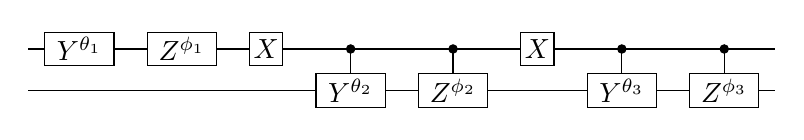
\begin{tikzpicture}[scale=1.000000,x=1pt,y=1pt]
\filldraw[color=white] (0.000000, -7.500000) rectangle (270.000000, 22.500000);
% Drawing wires
% Line 1: a W
\draw[color=black] (0.000000,15.000000) -- (270.000000,15.000000);
% Line 2: b W
\draw[color=black] (0.000000,0.000000) -- (270.000000,0.000000);
% Done with wires; drawing gates
% Line 3: a G $Y^{\theta_1}$ width=25
\begin{scope}
\draw[fill=white] (18.500000, 15.000000) +(-45.000000:17.677670pt and 8.485281pt) -- +(45.000000:17.677670pt and 8.485281pt) -- +(135.000000:17.677670pt and 8.485281pt) -- +(225.000000:17.677670pt and 8.485281pt) -- cycle;
\clip (18.500000, 15.000000) +(-45.000000:17.677670pt and 8.485281pt) -- +(45.000000:17.677670pt and 8.485281pt) -- +(135.000000:17.677670pt and 8.485281pt) -- +(225.000000:17.677670pt and 8.485281pt) -- cycle;
\draw (18.500000, 15.000000) node {$Y^{\theta_1}$};
\end{scope}
% Line 4: a G $Z^{\phi_1}$ width=25
\begin{scope}
\draw[fill=white] (55.500000, 15.000000) +(-45.000000:17.677670pt and 8.485281pt) -- +(45.000000:17.677670pt and 8.485281pt) -- +(135.000000:17.677670pt and 8.485281pt) -- +(225.000000:17.677670pt and 8.485281pt) -- cycle;
\clip (55.500000, 15.000000) +(-45.000000:17.677670pt and 8.485281pt) -- +(45.000000:17.677670pt and 8.485281pt) -- +(135.000000:17.677670pt and 8.485281pt) -- +(225.000000:17.677670pt and 8.485281pt) -- cycle;
\draw (55.500000, 15.000000) node {$Z^{\phi_1}$};
\end{scope}
% Line 5: a X
\begin{scope}
\draw[fill=white] (86.000000, 15.000000) +(-45.000000:8.485281pt and 8.485281pt) -- +(45.000000:8.485281pt and 8.485281pt) -- +(135.000000:8.485281pt and 8.485281pt) -- +(225.000000:8.485281pt and 8.485281pt) -- cycle;
\clip (86.000000, 15.000000) +(-45.000000:8.485281pt and 8.485281pt) -- +(45.000000:8.485281pt and 8.485281pt) -- +(135.000000:8.485281pt and 8.485281pt) -- +(225.000000:8.485281pt and 8.485281pt) -- cycle;
\draw (86.000000, 15.000000) node {$X$};
\end{scope}
% Line 6: b G $Y^{\theta_2}$ a width=25
\draw (116.500000,15.000000) -- (116.500000,0.000000);
\begin{scope}
\draw[fill=white] (116.500000, -0.000000) +(-45.000000:17.677670pt and 8.485281pt) -- +(45.000000:17.677670pt and 8.485281pt) -- +(135.000000:17.677670pt and 8.485281pt) -- +(225.000000:17.677670pt and 8.485281pt) -- cycle;
\clip (116.500000, -0.000000) +(-45.000000:17.677670pt and 8.485281pt) -- +(45.000000:17.677670pt and 8.485281pt) -- +(135.000000:17.677670pt and 8.485281pt) -- +(225.000000:17.677670pt and 8.485281pt) -- cycle;
\draw (116.500000, -0.000000) node {$Y^{\theta_2}$};
\end{scope}
\filldraw (116.500000, 15.000000) circle(1.500000pt);
% Line 7: b G $Z^{\phi_2}$ a width=25
\draw (153.500000,15.000000) -- (153.500000,0.000000);
\begin{scope}
\draw[fill=white] (153.500000, -0.000000) +(-45.000000:17.677670pt and 8.485281pt) -- +(45.000000:17.677670pt and 8.485281pt) -- +(135.000000:17.677670pt and 8.485281pt) -- +(225.000000:17.677670pt and 8.485281pt) -- cycle;
\clip (153.500000, -0.000000) +(-45.000000:17.677670pt and 8.485281pt) -- +(45.000000:17.677670pt and 8.485281pt) -- +(135.000000:17.677670pt and 8.485281pt) -- +(225.000000:17.677670pt and 8.485281pt) -- cycle;
\draw (153.500000, -0.000000) node {$Z^{\phi_2}$};
\end{scope}
\filldraw (153.500000, 15.000000) circle(1.500000pt);
% Line 8: a X
\begin{scope}
\draw[fill=white] (184.000000, 15.000000) +(-45.000000:8.485281pt and 8.485281pt) -- +(45.000000:8.485281pt and 8.485281pt) -- +(135.000000:8.485281pt and 8.485281pt) -- +(225.000000:8.485281pt and 8.485281pt) -- cycle;
\clip (184.000000, 15.000000) +(-45.000000:8.485281pt and 8.485281pt) -- +(45.000000:8.485281pt and 8.485281pt) -- +(135.000000:8.485281pt and 8.485281pt) -- +(225.000000:8.485281pt and 8.485281pt) -- cycle;
\draw (184.000000, 15.000000) node {$X$};
\end{scope}
% Line 9: b G $Y^{\theta_3}$ a width=25
\draw (214.500000,15.000000) -- (214.500000,0.000000);
\begin{scope}
\draw[fill=white] (214.500000, -0.000000) +(-45.000000:17.677670pt and 8.485281pt) -- +(45.000000:17.677670pt and 8.485281pt) -- +(135.000000:17.677670pt and 8.485281pt) -- +(225.000000:17.677670pt and 8.485281pt) -- cycle;
\clip (214.500000, -0.000000) +(-45.000000:17.677670pt and 8.485281pt) -- +(45.000000:17.677670pt and 8.485281pt) -- +(135.000000:17.677670pt and 8.485281pt) -- +(225.000000:17.677670pt and 8.485281pt) -- cycle;
\draw (214.500000, -0.000000) node {$Y^{\theta_3}$};
\end{scope}
\filldraw (214.500000, 15.000000) circle(1.500000pt);
% Line 10: b G $Z^{\phi_3}$ a width=25
\draw (251.500000,15.000000) -- (251.500000,0.000000);
\begin{scope}
\draw[fill=white] (251.500000, -0.000000) +(-45.000000:17.677670pt and 8.485281pt) -- +(45.000000:17.677670pt and 8.485281pt) -- +(135.000000:17.677670pt and 8.485281pt) -- +(225.000000:17.677670pt and 8.485281pt) -- cycle;
\clip (251.500000, -0.000000) +(-45.000000:17.677670pt and 8.485281pt) -- +(45.000000:17.677670pt and 8.485281pt) -- +(135.000000:17.677670pt and 8.485281pt) -- +(225.000000:17.677670pt and 8.485281pt) -- cycle;
\draw (251.500000, -0.000000) node {$Z^{\phi_3}$};
\end{scope}
\filldraw (251.500000, 15.000000) circle(1.500000pt);
% Done with gates; drawing ending labels
% Done with ending labels; drawing cut lines and comments
% Done with comments
\end{tikzpicture}

	\end{center}
	Takes $\mathcal{O}(2^n)$ gates, so linear in the number of data points.
\end{frame}

\begin{frame}{Measure coefficients}
	\pause
	\begin{itemize}
		\item Three step process:
		\begin{itemize}
			\item Measuring the amplitudes by computational basis measurements.
			\item Measure absolute value of relative phases by first applying $H$ to one of the qubits.
			\item Measure sign of relative phases by first applying $S$ and $H$ to one the qubits.
		\end{itemize} \pause
		\item Takes $\mathcal{O}(2^n)$ number of measurements, i.e., linear in the number of data points.
	\end{itemize}
\end{frame}

\begin{frame}{Demo}
	\includegraphics[width=.45\textwidth]{elephant.png} \hfill
	\includegraphics[width=.45\textwidth]{batman.png}
\end{frame}

\begin{frame}{Conclusion}
	\pause
	\begin{itemize}
		\item No real speed-up here. \pause
		\item Useful for benchmarking.
	\end{itemize}
\end{frame}